\documentclass[12pt, oneside, a4paper]{book}
\usepackage{setspace}
\usepackage{arabtex}
\usepackage{utf8} 
\usepackage{hyperref} 
\usepackage{graphicx}
\usepackage{subcaption}
\usepackage{geometry}
\usepackage{lipsum}
\usepackage{listings}
\usepackage{xcolor}
\usepackage{enumitem}
\usepackage{titlesec}
\usepackage{xparse}
\usepackage{verbatim}
\usepackage{float}
\usepackage{array}
\usepackage{ragged2e}
\usepackage{tabularx}
\usepackage{verbatimbox}
\usepackage{fancyhdr}
 \geometry{a4paper,inner=1.25in,outer=1.25in,top=1in,bottom=1in,footskip=15mm,headsep=5mm,headheight=15mm}
% \renewcommand{\chaptermark}[1]{\markboth{\textit{\uppercase{chapter \thechapter. #1}}}{}}

\titlespacing*{\chapter}{0pt}{-\baselineskip}{1em}
\pagestyle{fancy} % Turn on the style
\renewcommand{\headrulewidth}{0pt}

\fancyhf{} % Start with clearing everything in the header and footer
\rhead{
	{\tiny \RL{المملكة العربية السعودية} \\
		\RL{وزارة التعليم العالي} \\
		\RL{جامعة الأميرة نورة بنت عبد الرحمن} \\
		\RL{كلية علوم الحاسب والمعلومات} \\
		\RL{مشروع تخرج ١}}
}
\chead{
\includegraphics[width=.1\linewidth]{img/pnu.png}}
\lhead{
	{\tiny Kingdom of Saudi Arabia \\
		Ministry of Higher Education \\
		Princess Nourah bint Abdulrahman University \\
		Faculty of Computer \& Informaion Science \\
		Graduation Project I}
}
\cfoot{\thepage}%

\fancypagestyle{plain}
{
	\rhead{
		{\tiny \RL{المملكة العربية السعودية} \\
			\RL{وزارة التعليم العالي} \\
			\RL{جامعة الأميرة نورة بنت عبد الرحمن} \\
			\RL{كلية علوم الحاسب والمعلومات} \\
			\RL{مشروع تخرج ١}}
	}
	\chead{
\includegraphics[width=.1\linewidth]{img/pnu.png}}
	\lhead{
		{\tiny Kingdom of Saudi Arabia \\
			Ministry of Higher Education \\
			Princess Nourah bint Abdulrahman University \\
			Faculty of Computer \& Informaion Science \\
			Graduation Project I}
	}
	\cfoot{\thepage}%
}
\fancypagestyle{firstpage}
{
	\rhead{
		{\tiny \RL{المملكة العربية السعودية} \\
		\RL{وزارة التعليم العالي} \\
		\RL{جامعة الأميرة نورة بنت عبد الرحمن} \\
		\RL{كلية علوم الحاسب والمعلومات} \\
		\RL{مشروع تخرج ١}}
	}
	\chead{
\includegraphics[width=.1\linewidth]{img/pnu.png}}
	\lhead{
		{\tiny Kingdom of Saudi Arabia \\
		Ministry of Higher Education \\
		Princess Nourah bint Abdulrahman University \\
		Faculty of Computer \& Informaion Science \\
		Graduation Project I}
	}
}
\usepackage{xpatch}
\xapptocmd{\titlepage}{\thispagestyle{firstpage}}{}{}

\newcommand{\mychapter}[1]{\newpage%
	\thispagestyle{empty}
	\topskip0pt%
	\vspace*{\fill}%
	\addtocounter{chapter}{1}%
	\begin{center}%
		\textbf{\Large{\color{section}{CHAPTER NO. \thechapter \\ \uppercase{#1}}}}%
	\end{center}%
	\vspace*{\fill}%
	\addtocounter{chapter}{-1}
	\newpage%
	\chapter{#1}
}


\definecolor{section}{HTML}{86496b}
\definecolor{chapter}{HTML}{ff7468}
\definecolor{sub}{HTML}{547a87}
\definecolor{ssub}{HTML}{97d0c0}
\definecolor{bold}{HTML}{ffca2e}


\definecolor{lightgray}{HTML}{eeeeee}
\definecolor{darkgray}{rgb}{.4,.4,.4}
\definecolor{purple}{rgb}{0.65, 0.12, 0.82}
\definecolor{green}{rgb}{0,0.6,0}


\titleformat{\chapter}
{\color{chapter}\normalfont\Large\bfseries}
{\color{chapter}\thechapter}{1em}{}

\titleformat{\section}
{\color{sub}\normalfont\fontsize{12}{16}\bfseries}
{\color{sub}\thesection}{1em}{}

\titleformat{\subsection}
{\color{section}\normalfont\fontsize{12}{14}\bfseries}
{\color{section}\thesubsection}{1em}{}

\titleformat{\subsubsection}
{\color{ssub}\normalfont\fontsize{12}{13}\bfseries}
{\color{ssub}\thesubsubsection}{1em}{}



\newcommand\boldcolor[1]{\textcolor{bold}{\textbf{#1}}}
\newcommand\Includegraphics[2][]{\addvbuffer[3pt 0pt]{\includegraphics[#1]{#2}}}

\lstset{frame=tb,
	language=Java,
	aboveskip=3mm,
	belowskip=3mm,
	showstringspaces=false,
	columns=flexible,
	basicstyle={\small\ttfamily},
	numbers=none,
	numberstyle=\tiny\color{gray},
	keywordstyle=\color{blue},
	commentstyle=\color{dkgreen},
	stringstyle=\color{mauve},
	breaklines=true,
	breakatwhitespace=true,
	tabsize=3
}
\setcounter{secnumdepth}{3}
\setcounter{tocdepth}{3}
\hypersetup{
	colorlinks,
	citecolor=[rgb]{0,0.5,0.5},
	filecolor=[rgb]{0,0.5,0.5},
	linkcolor=[rgb]{0,0.5,0.5},
	urlcolor=[rgb]{0,0.5,0.5}
}

\date{}
\title{
	\color{chapter}
	Online Home Automation Control System \\
	\color{black}\large 2019-2020 Graduation Project I}

\author{
	\setcode{utf8}
	\RL{ريم علي الغامدي} 
	\\\texttt{437004875}
	\\[3ex]
	\RL{ساره خالد آل حسين} 
	\\\texttt{436006939}
	\\[3ex]
	\RL{ضحى نضال الزعبي} 
	\\\texttt{436200063}
	\\[3ex]
	\RL{عبير أحمد عزت} 
	\\\texttt{436200058}
	\\[3ex]
	\RL{منى سعود الخثلان} 
	\\\texttt{437004005}
	\\[3ex]
	\RL{نوف عبد الله الدعجاني} 
	\\\texttt{437004100}
	\\	\\
	\Large\RL{د. عبير محمود} 
}
\begin{document}
	
	
	\pagenumbering{gobble}
	\maketitle
	\newpage

	\addcontentsline{toc}{chapter}{Acknowledgement}
	\pagenumbering{roman}

	\addcontentsline{toc}{chapter}{Table of Contents}\tableofcontents
	\newpage	
	\doublespacing
	\newpage
	
	\addcontentsline{toc}{chapter}{List of Tables}
	\listoftables
	\newpage
	
	\addcontentsline{toc}{chapter}{List of Figures}
	\listoffigures
	\newpage
	
	\addcontentsline{toc}{chapter}{\nameref{sec:sym}}
	\chapter*{List of Symbols \& Abbreviations}
	\markboth{\uppercase{List of Symbols \& Abbreviations}}{}
	\label{sec:sym}
	\def\arraystretch{1.5}
	\begin{table}[H]
		\caption{List of Symbols \& Abbreviations}
		\begin{center}
			\begin{tabularx}{\linewidth}{|c|X|}\hline
				
				\boldcolor{Symbols \& Abbreviations} & \boldcolor{Meaning} \\\hline
				UI & User Interface\\\hline
				API & Application programming Interface\\\hline
				GPIO & General Purpose Input Output\\\hline
				IDE & Integrated Development Environment \\\hline
				IoT & Internet of Things \\\hline
				LED & Light Emitting Diode\\\hline
				REST & Representational State Transfer\\\hline
				SDLC & Software Development Life Cycle\\\hline
				SQL & Structured Query Language\\\hline
			\end{tabularx}
		\end{center}
	\end{table}

	\addcontentsline{toc}{chapter}{\nameref{sec:intro}}
	\chapter*{Abstract \& Keywords}
		\markboth{\uppercase{Abstract \& Keywords}}{}
		\label{sec:intro}
		\paragraph{} The aim for this project is to control lights, air conditioners, television or any other home appliance regardless of the person's location. The methodology is simple: an android app will send controlling requests to a web server. Raspberry Pi will be getting all the new requests from the server, processing it accordingly and controlling the hardware components connected to it. Such a system will allow someone in the United States to turn the lights in their house in Saudi Arabia on. However, an active connection to the internet must be present all the time. \\ \\
		\def\arraystretch{1.5}
		\begin{table}[H]
			\caption{Keywords}
			\begin{center}
				\begin{tabularx}{\linewidth}{|c|X|}\hline		
					\boldcolor{Keyword} & \boldcolor{Definition} \\\hline
					Raspberry Pi & low cost, credit-card sized computer\cite{raspberry}. \\\hline
					Linear solenoid &  type of electromagnetic actuator that converts an electrical signal into a magnetic field producing a linear motion\cite{linear}.\\\hline				
				\end{tabularx}
			\end{center}
		\end{table}
	

	\mychapter{Introduction}
		\pagenumbering{arabic}
		\section{Problem statement \& Significance}
		\paragraph{}With the recent very rapid progress in technology and automation, there has become a need for remote control of almost all possible aspects of living, especially the house appliances that surround us, because of how easy it makes the modern human’s life and how much it allows them to focus on their main work and be more productive instead of doing these remotely controlled tasks for themselves, and simply, of how convenient it is. Examples we have already encountered and used in our daily lives include using apps to control a cleaning robot or adjust the heating in the house or even make coffee or switch the house lights on or off. For the latter, there have been many applications that can do that, however they all work locally and there hasn’t been one yet that uses the internet so it can be used remotely from outside the house to control the lights. It is necessary for an application like that to exist, as a service like this would be important for many people, like, for example, working moms who are outside the house and want to switch the lights on at a certain time to wake their children up, or pet owners who need to have UV lights switched on for their pets at certain times of the day but can’t do so immediately and so on. However, the main challenge in creating a device to solve this problem is where the idea of IoT (Internet of Things) comes in; learning how to control this device through the Internet from afar, rather than being controlled by infrared rays locally as is the case with most similar applications.
		\section{Proposed Solution}
		\paragraph{}The created app should enable the user, by clicking on the appropriate buttons, to control a physical apparatus in the building where the lights are and have the lights turn on or off accordingly. This will be done by designing and creating an Android application, then using a small laptop, called Raspberry Pi, to control a small piece that will be pushed forward (on command) to switch the light on or off, the API is a web application hosted on a server.
		
		\subsection{Aims}
			\paragraph{}At the end of this project, we intend to achieve the following aims:
			\begin{itemize}
	 			\item Learn how to design a mobile application using previously learned and new knowledge
				\item Learn how to invoke a web API and use it in our application
				\item Learn Python programming language to control Raspberry Pi
				\item Learn Flask web micro-framework
			\end{itemize}
		\subsection{Goals}
			\paragraph{} At the end of this project, we expect to deliver:
			\begin{itemize}
				\item An Android application with a user friendly, simple, clear interface with buttons to control a LED and linear solenoid.
				\item A physical apparatus composed of the Raspberry Pi connected to and controlling the piece.
				\item A web application following REST architecture, managing user  requests and Raspberry Pi's responses.
			\end{itemize}
		\section{Project Domain \& Limitation}
			\subsection{Domain}
				\paragraph{} Although the application will be available for all kinds of users to use, we expect that the ones who would make the most use of it would be employees who have long working hours and would need to be able to remotely control appliances in their homes, especially lights.
				\paragraph{} The critical piece in all of this application would be the linear solenoid actuator i.e. the small electrically controlled piece that would be placed very close to the light switch and would, on command, spring forward to press on the switch to turn it on or off. 
			\subsection{Limitation}
			\paragraph{} The main limitation of the application is that it will be able to control only a limited type of home appliance, which is the lights. A much more advanced application would be able to control most of the other appliances, such as controlling an Air conditioner if the owner is outside, or a timer controlled coffee maker.
			
		\section{Gantt Chart}
		\begin{figure}[H]
  			\caption{Gantt Chart}
			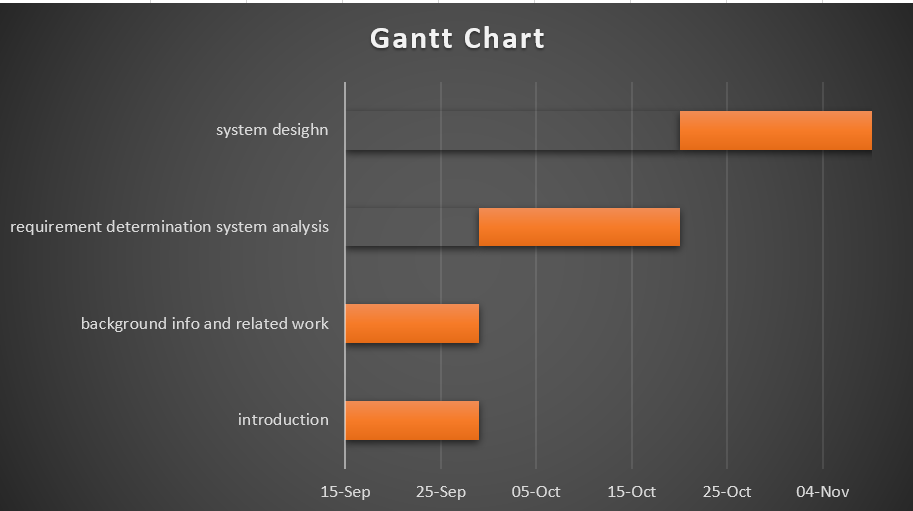
\includegraphics[width=\linewidth]{img/gantt_chart.png}
		\end{figure}
		\newpage	
		\mychapter{Background Information \& Related Work}
			\section{Background Information}
			\subsection{IoT}
			\paragraph{}The internet of things (IoT) constitutes one of the most important technological
			development in the last decade. The IoT term was coined by Kevin n 1999\cite{iot_1}. IoT
			means a “world-wide network of interconnected objects uniquely addressable, based
			on standard communication protocols”\cite{iot_2}. in a somewhat simplified manner, we
			can describe IoT is the ability to connecting as many things by the internet without
			direct human intervention by using technologies such as cloud computing, Radio
			Frequency Identification (RFID), wireless communication, sensors, Internet
			protocol, ultra-low-power processors and others\cite{iot_3}.
			\subsubsection{IoT Architecture}
			\paragraph{} IoT Architecture includes three layers Perception layer, Network layer, and
			Application layer each of them has its own functionality.
			\begin{itemize}
				\item \boldcolor{Perception layer:} is responsible to perceive and identifying objects or things in the
				environment.
				\item \boldcolor{Network layer:} is responsible for receiving and transmitting data between layers.
				\item \boldcolor{Application layer:} is the interface for all previous Layers used to processed and
				transported data to provide services to the users\cite{iot_4}.
			\end{itemize}
			\subsubsection{IoT Applications:}
			\paragraph{}The Applications of the IoT are diversified and can be classified into three main
			categories industry, environment, and society.
			\begin{itemize}
			\item \boldcolor{Industry:} The importance of the industry domain can be seen in transportation,
			aviation, and automotive (e.g.Tesla automobile ).
			\item \boldcolor{Environment:} The society Domain focused on telecommunication, smart building,
			home, and medical technology (e.g.connected door locks, Closed-loop (automated)
			insulin delivery).
			\item \boldcolor{Society:} The environment Domain focused on recycling, disaster alerting,
			environmental monitoring (e.g.Forest Fire Detection, Air Pollution)\cite{iot_5}.
			\end{itemize}
			\subsection{Hardware}
				\begin{itemize}
				\item \boldcolor{Raspberry Pi:} a small general purpose computer. All hardware components will be connected to it. An active connection to the internet is needed for it to fetch data from the server. %insert figure here% 
				\item \boldcolor{Ubuntu Web Server:} hosts the web application. Digital Ocean severs were chosen for this project.
				
				\item \boldcolor{LED:} since the hardware components controlled depends heavily on the user needs, this project main aim will be controlling a small LED. LED stands for light-emitting diode. Basically a small light source. %insert figure here% %
				\item \boldcolor{Linear Solenoid:} once the LED works, linear solenoid will be installed for demonstrating the idea. It is a small component that generates a linear motion. It will be used to press in anything, such as lights, TV remote, and coffee machine. %insert figure here%
				\end{itemize}
				
			\subsection{Programming Languages \& Frameworks}
				\begin{itemize}
					
					\item \boldcolor{Python:} raspberry pi can be controlled by either c++ or python. Python was chosen because a REST API can be made using it fast.
		 				\begin{itemize}
		 					\item \textbf{GPIO:} a library for controlling any hardware component connected to the GPIO pins.
		 					\item \textbf{Flask:} a lightweight framework to build web applications.
						\end{itemize}
					\item \boldcolor{Java:} mobile application are made in a native way with either swift or java.
						\begin{itemize}
							\item \textbf{Android:} a framework for making android apps.
							\item \boldcolor{Retrofit:} type-safe HTTP client for Android and Java. It will be used to send and receive commands and status from the web server.
							
						\end{itemize}
					\item \boldcolor{PostgreSQL:} an open-source RDBMS. It will be installed on the server.
				\end{itemize}
			
			\subsection{SDLC Model}
			\paragraph{} Incremental model will be used in this project. This model is a process of software development where requirements are broken down into multiple standalone modules of software development cycle. Incremental development is done in steps from analysis design, implementation, testing / verification, maintenance\cite{sdlc}. The reason this model was chosen is the pieces will be installed, tested and connected to the system gradually. First a LED, then a linear solenoid and so on.
			
			
		\newpage	
		\section{Related Work}
		\subsection{Insteon - Insteon Hub}
		\begin{figure}[H]
  			\caption{Related Work: Insteon}
			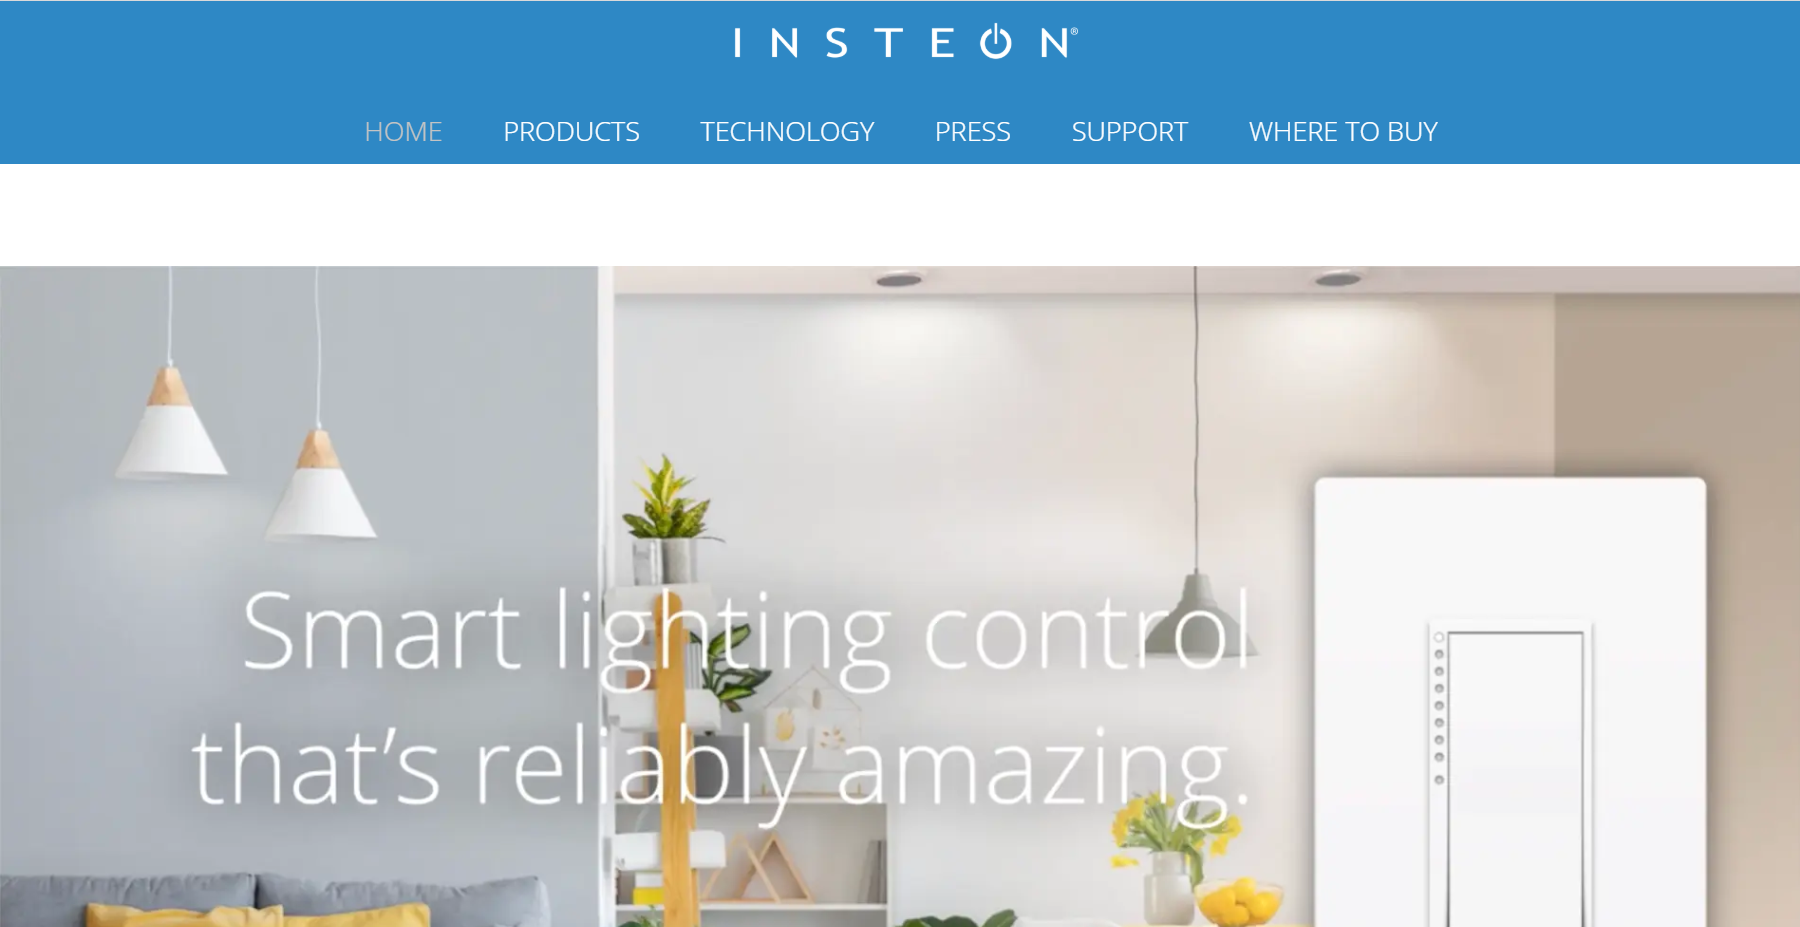
\includegraphics[width=\linewidth]{img/insteon.png}
		\end{figure}
		\paragraph{}Insteon Hub is a simple and straightforward device that connects you to your home from any smartphone or tablet, anywhere in the world. Control Insteon light bulbs, wall switches, outlets, and thermostats at home or remotely and receive instant email or push notification alerts from motion, door and window, water leak, and smoke sensors while you’re away\cite{insteon}.
		\begin{itemize}
		\item \boldcolor{Advantage:}
			\begin{enumerate}
				\item Control Multiple Devices Simultaneously with a Basic Scene.
				\item Create Schedules to Turn Your Lights On and Off at Specific Times.
				\item Automatically Turn Lights On and Off with Sensors.
				\item Monitor Your Home with Email or Push Notification Alerts.
			\end{enumerate}
		\item \boldcolor{Disadvantage:} 
			\begin{enumerate}
				\item Hub setup takes a couple of minutes and a few moments per light switch, sensor.
				\item Its need to connect it to power and your home's internet router so if the internet die all devices need to start over again. 
				\item fixed the hub take more cost than its original price.
				\item There is no database save/restore. You have to recreate all the devices, scenes, schedules if its replaced.
			\end{enumerate}
		\end{itemize}
		\newpage	
		\subsection{Wink - Wink Hub 2}
		\begin{figure}[H]
  			\caption{Related Work: Wink}
  			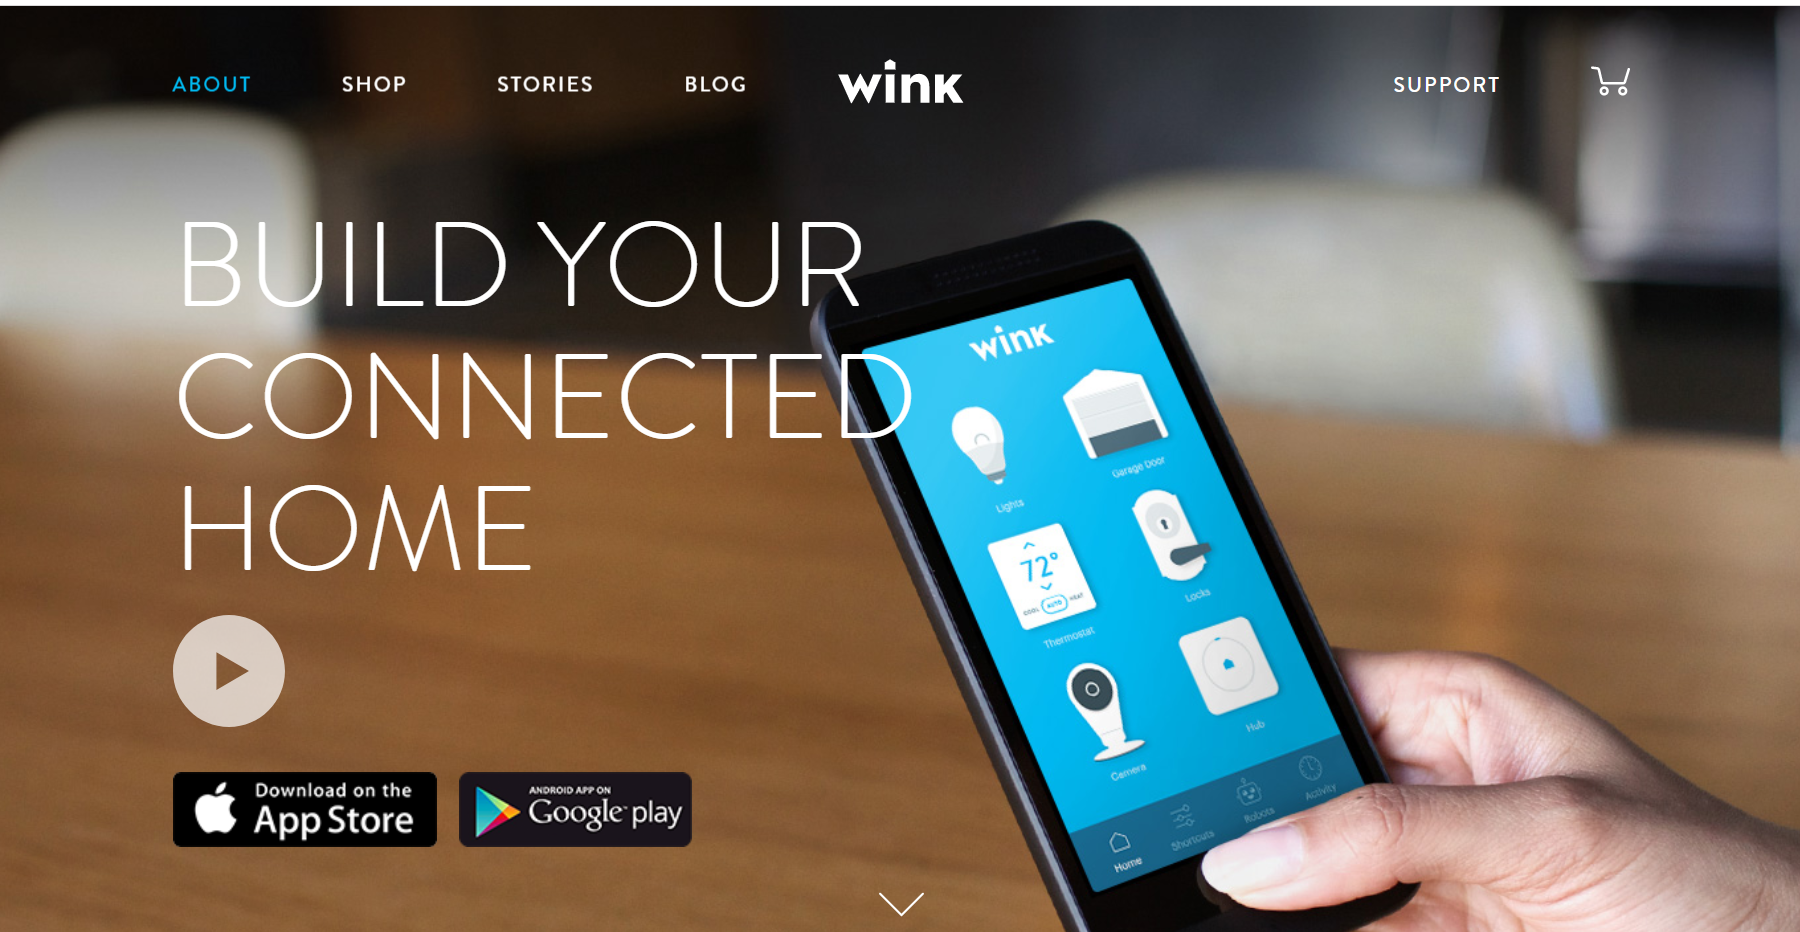
\includegraphics[width=\linewidth]{img/wink.png}
		\end{figure}
		\paragraph{}Wink Hub 2 is the world’s first smart home hub created for the mainstream consumer. With industry-leading smart home protocol support, enhanced connectivity features, and a sleek design, Wink Hub 2 brings hundreds of products from best-in-class brands together for a simple, intuitive experience\cite{wink}.
		
		\begin{itemize}
			\item \boldcolor{Advantage:}
			\begin{enumerate}
				\item Support Different platforms such as iOS or Android.
				\item Once you've created an account, Wink has the ability to recognize the products within Wink Bright, guide you through a few simple steps, and then you're ready to go.
				\item Wink works with Cortana Microsoft’s voice assistant and Amazon Alexa.
				\item One Important features in wink, its can see what you’re spending even before the bill arrives.
			\end{enumerate}
			\item \boldcolor{Disadvantage:} 
			\begin{enumerate}
				\item One major problem with the Wink 2 hub is that the device sometimes loses connectivity and must be reset in order for it to connect again.
				\item Wink app doesn't always let you access other devices' full features.
				\item High price.
				\item Takes 14 days to arrive.
			\end{enumerate}
		\end{itemize}
		\newpage
		\subsection{Samsung – Smart Things Hub}
		\begin{figure}[H]
  			\caption{Related Work: Samsung}
			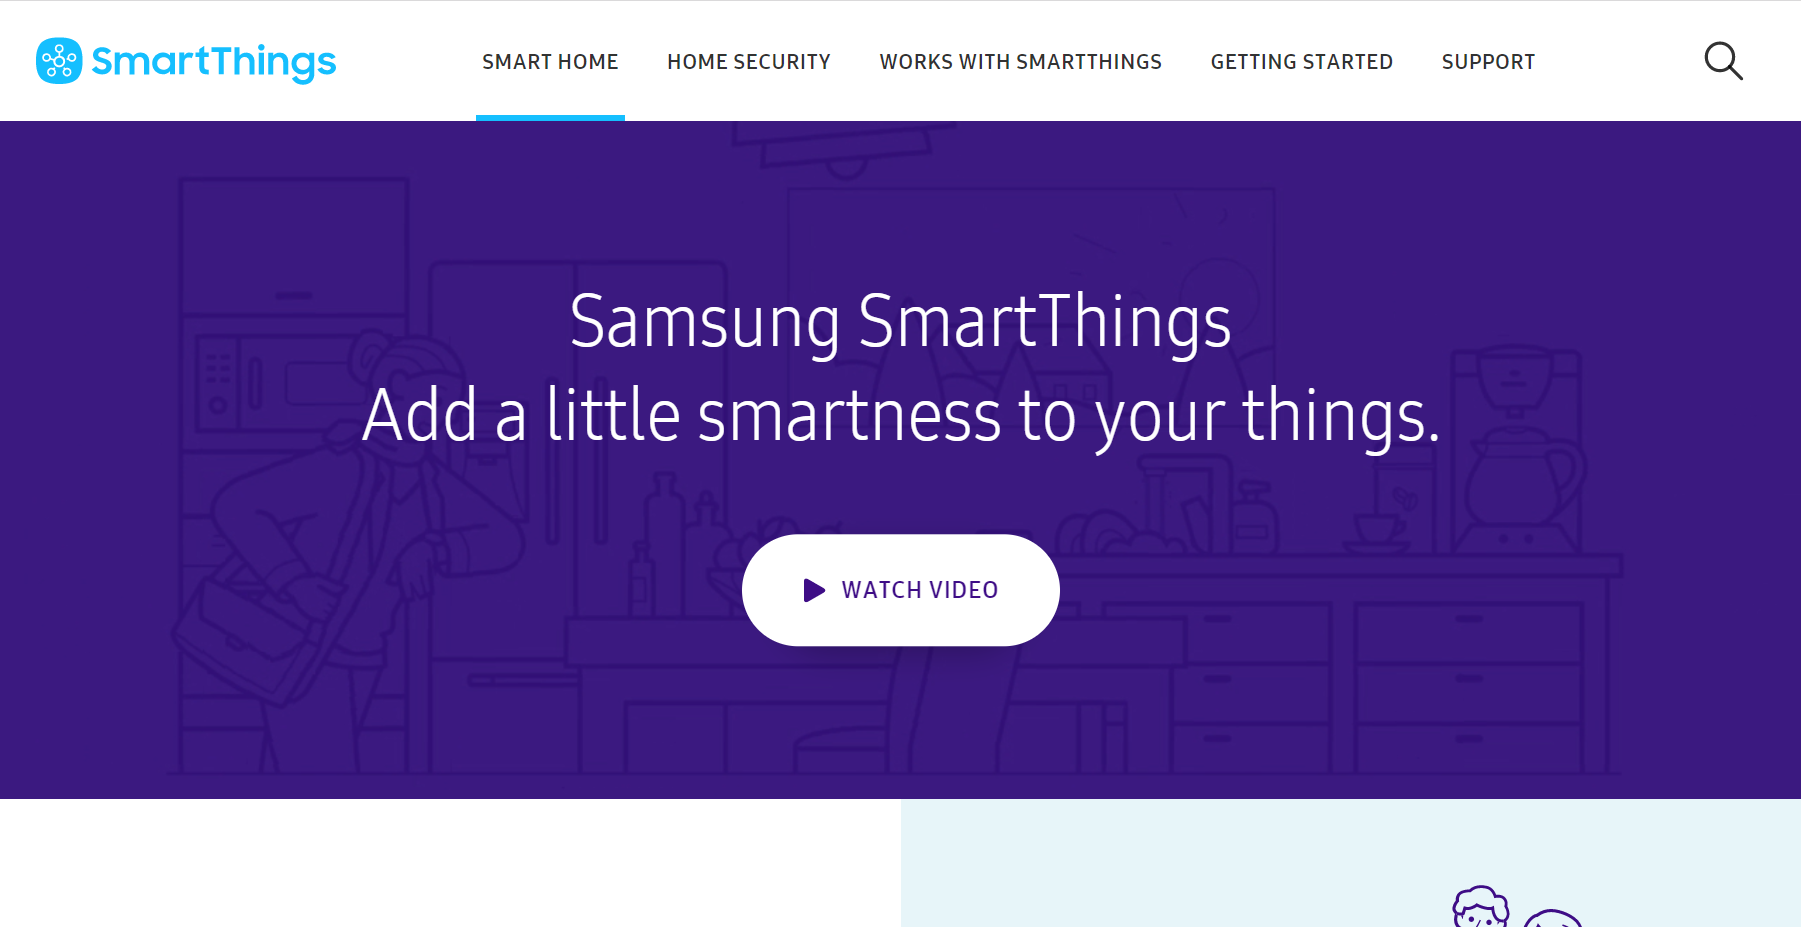
\includegraphics[width=\linewidth]{img/samsung.png}
		\end{figure}
		\paragraph{}Smart things hub Connect wirelessly with a wide range of smart devices and make them work together\cite{samsung}.
		\begin{itemize}
			\item \boldcolor{Advantage:}
			\begin{enumerate}
				\item Monitor and control connected devices in your home using a single SmartThings app for iPhone or Android.
				\item Manage connected devices in your home with SmartThings Routines for Good Morning, Goodbye, Good Night, and more.
				\item Receive alerts from connected devices when there’s unexpected activity in your home.
				
			\end{enumerate}
			\item \boldcolor{Disadvantage:} 
			\begin{enumerate}
				\item Some compatible components may not work as efficiently or smoothly as you want them to, which may be inconvenient.
				\item Some users report it stops working at times.
				\item Difficult to upgrade from older hub.
				\item In US Only.
			\end{enumerate}
		\end{itemize}
		\section{Proposed \& Similar System Comparison}
			\def\arraystretch{1.5}
			\begin{table}[H]
				\caption{Proposed \& Similar System Comparison}
			\begin{center}
			\begin{tabularx}{\linewidth}{|m{4cm}*4{|X}|}\hline
					
					& \boldcolor{Raspberry Pi} & \boldcolor{Insteon} & \boldcolor{Wink hub 2} & \boldcolor{Samsung (smart things)}  \\\hline
					
					\boldcolor{design} &
						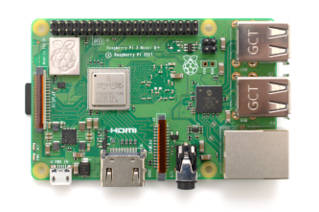
\includegraphics[width=\linewidth]{img/raspberry.png} &
						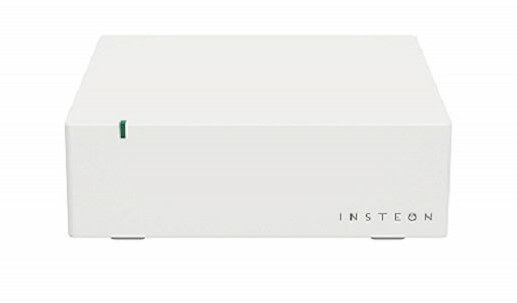
\includegraphics[width=\linewidth]{img/insteon_hw.png} & 
						\Includegraphics[width=\linewidth]{img/wink_hw.png} &
						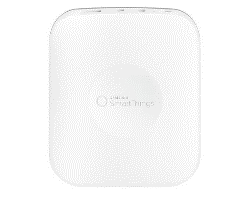
\includegraphics[width=\linewidth]{img/samsung_hw.png}
					 \\\hline
					\boldcolor{Works With Wi-Fi} & yes & yes & yes & yes  \\\hline


					
					\boldcolor{Parts Price} & very cheap & expensive & very expensive & expensive  \\\hline
					\boldcolor{Price} & 25\$ & 80\$ & 99\$ & 70\$ \\\hline
					
					\boldcolor{Installation \& Configuration Difficulty} & hard to install but doesn't takes time to reinstall and configure& easy to install and hardly takes any time setting up even if you change your home  & easy to install and hardly takes any time setting up even if you change your home  & easy to install and hardly takes any time setting up even if you change your home
					\\\hline
				\end{tabularx}
			\end{center}
		\end{table}
		\newpage	

	\mychapter{System Analysis}
		\section{Requirement Specification}
			\subsection{Overview}
				\paragraph{} The application we mean to create consists of three main systems: the android application which will be the user interface, the Raspberry Pi, which is the small computer where all the hardware pieces will be connected to, and the web server which will host the REST web application and be the connection between the android application and the Raspberry Pi.
				\paragraph{}The user of the system will have to have the android app installed on his mobile phone. When the app is first opened, the first activity (page in android app) displays the hardwares that are connected to the Raspberry Pi. It gets this list of hardwares from the webserver by using the GET method. When the user clicks on any of the hardware that is there, a new activity opens. In it is mentioned the name of the hardware, the status (e.g. whether it is on or off), the commands and the scheduling configuration. All of this information is obtained from the server. 
				\paragraph{}Next to the commands title, there will be a small button that when clicked on will open a third activity, which gives the option of adding a new command. The command can be instantaneous (for example, switching an LED light immediately) or it can be scheduled for a later date or time. For the instantaneous command, the POST method will be used, and for scheduling the commands, the user will have the option to choose the date and time he wishes the commands to be undertaken in. Whatever the outcome of this process is, a popup message will appear to the user either confirming the success of the command the user issued, or denying it while explaining the reason for that failure.
				\paragraph{}Under the commands tab, there will be a  configuration 	section where all the scheduled commands will appear, along with their dates and times and options to edit them or delete them. The edit option will be done by the PUT method and the deleted option by the DELETE method. All the methods work on the data in the server’s database i.e. they either add a new command (POST), edit a scheduled command (PUT), or delete an existing command (DELETE). 
				\paragraph{}For the Raspberry Pi, the sequence it works according to is timed. Every 5 minutes, it puts the hardware status to the server so that it can show on the user’s application hardware list. Also, every 30 seconds, it checks the server for any new commands posted by the user from the android application. If there are any new ones that have to be, it updates its own local database (an action queue) according to the priorities and scheduled dates and times of the commands. This local database is organized according to the time the command was issued (i.e. the instantaneous commands are put at the front of this queue because of their precedence and the scheduled ones are put in the command order) and contains the command ID, which hardware this command was issued for, when this command was issued, and whether the command was successfully done or not, all gotten from the server by the GET method except the “successfully done” column, which the Raspberry edits according to the hardware. 
				\paragraph{}Whatever the result of the command was, the Raspberry posts the response of the command to the server. The android application gets this response from the server every 5 or 10 minutes, depending on the user’s choice. The response is displayed as a push notification in the user’s mobile phone. Depending on this response, the status and configuration information in the app will be updated to reflect the success or failure of the command response. Finally, it is important to note that any new hardware or configuration added to or connected to the Raspberry will have its information posted to the server by the Raspberry computer, where the user can view it then as soon as he opens his application to the first activity.
				
				\subsubsection{Input}
				The user command issued using the Android client is the main input. Each command consist of the following:
				\begin{itemize}
					\item chosen hardware.
					\item configuration wanted.
					\item optional scheduling information.
				\end{itemize}
				The \textbf{hardware} is the physical component connected to raspberry pi. Each hardware has a set of possible states that it can be in. Those states are called \textbf{configuration}. The \textbf{schedule} indicates the time of day and days of week the user might want the command to run at.
				\subsubsection{Output}
				\begin{itemize}
					\item a respond
				\end{itemize}
				The raspberry pi issues a \textbf{respond} indicating whether the command has been successfully done with an optional message. This respond is saved in the webserver, which in turn is read by the android client periodically.  
			
		\newpage\section{Requirement Analysis}
			\subsection{Software Requirements}
			\newpage\subsection{Hardware Requirements}
				\begin{itemize}
					\item \boldcolor{Raspberry Pi} 
					\begin{itemize}
						\item Raspberry Pi 3 B+.
						\item a minimum of 2 GB of RAM.
						\item a minimum of 10 GB space in SD card.
						\item a monitor, a keyboard and a mouse, alternatively SSH connection could be established.
						\item internet connection, either via Wi-Fi or Ethernet cable.
						\item breadboard, cables, and resistors for circuit.
						\item RGB LED, solenoid, or any other hardware components satisfying user needs.
					\end{itemize}
					\item \boldcolor{Web Server} 
					\begin{itemize}
						\item Ubuntu 16.04+ web server, we chose digital ocean's.
						\item Minimum of 1GB of RAM.
						\item Minimum of 10GB of available space.
					\end{itemize}
					\item \boldcolor{Android mobile phone} 
				\end{itemize}
			\newpage\subsection{Functional Requirements}
			\newpage\subsection{Non-Functional Requirements}
				\def\arraystretch{1.5}
				\begin{table}[H]
					\caption{Non-functional requirements}
					\begin{center}
						\begin{tabularx}{\linewidth}{|c|X|}\hline
							\boldcolor{Requirement} & \boldcolor{Description}\\\hline
							\textbf{Availability} & The system shall not be shut down for maintenance for more than 1 minute. \\\hline
							\textbf{Usability} & The user shall be able to learn the most important 5 functions of application in 2 hours.  \\\hline
							\textbf{Verifiability} & When a new version of the main system is released, it shall be possible to upgrade to it from any previous version. \\\hline
							\textbf{Performance} & Any interface between a user and the automated system shall have a maximum response time of three seconds. \\\hline
							\textbf{Flexibility} & Application shall be made of multiple languages. So, user shall be able to nominate their preferred language when entering their personal information. \\\hline
						\end{tabularx}
					\end{center}
				\end{table}
			\newpage\subsection{Structured Diagrams}
				\subsubsection{Use Case Diagram}
					\begin{figure}[H]
					\caption{Use case diagram}
					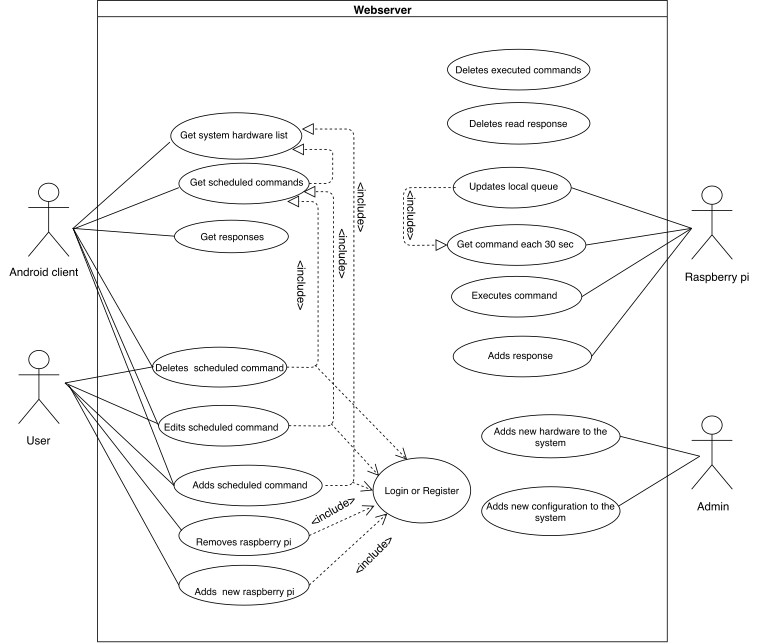
\includegraphics[width=\linewidth]{img/diagram_usecase.jpg}
					\end{figure}
				
				\newpage\subsubsection{Use Case Scenarios}
				\newpage\subsubsection{Flowchart Diagram}
				\newpage\subsubsection{Entity Relationship Diagram}
					\begin{figure}[H]
						\caption{Entity-relationship diagram}
						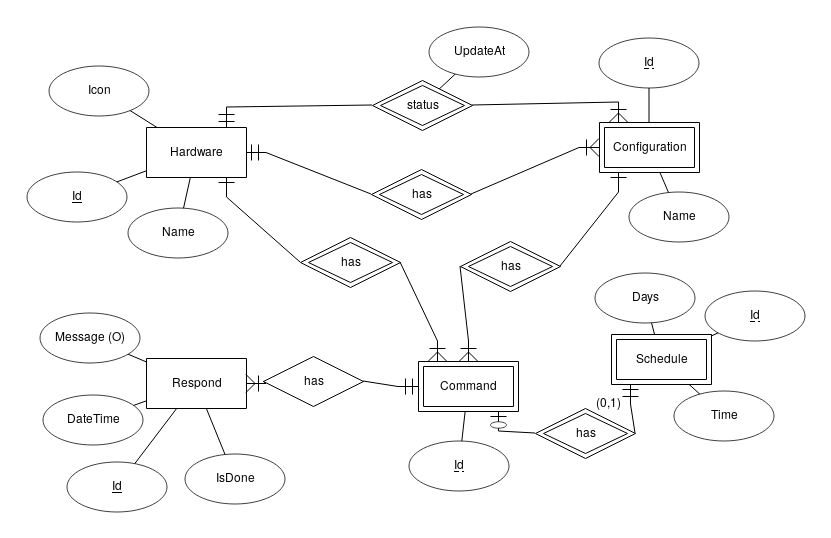
\includegraphics[width=\linewidth]{img/diagram_er.png}
					\end{figure}
				
			\newpage\subsection{Object-Oriented Diagrams}
				\subsubsection{Sequence Diagrams}
				\newpage\subsubsection{Class Diagram}
					\begin{figure}[H]
						\caption{Class diagram}
						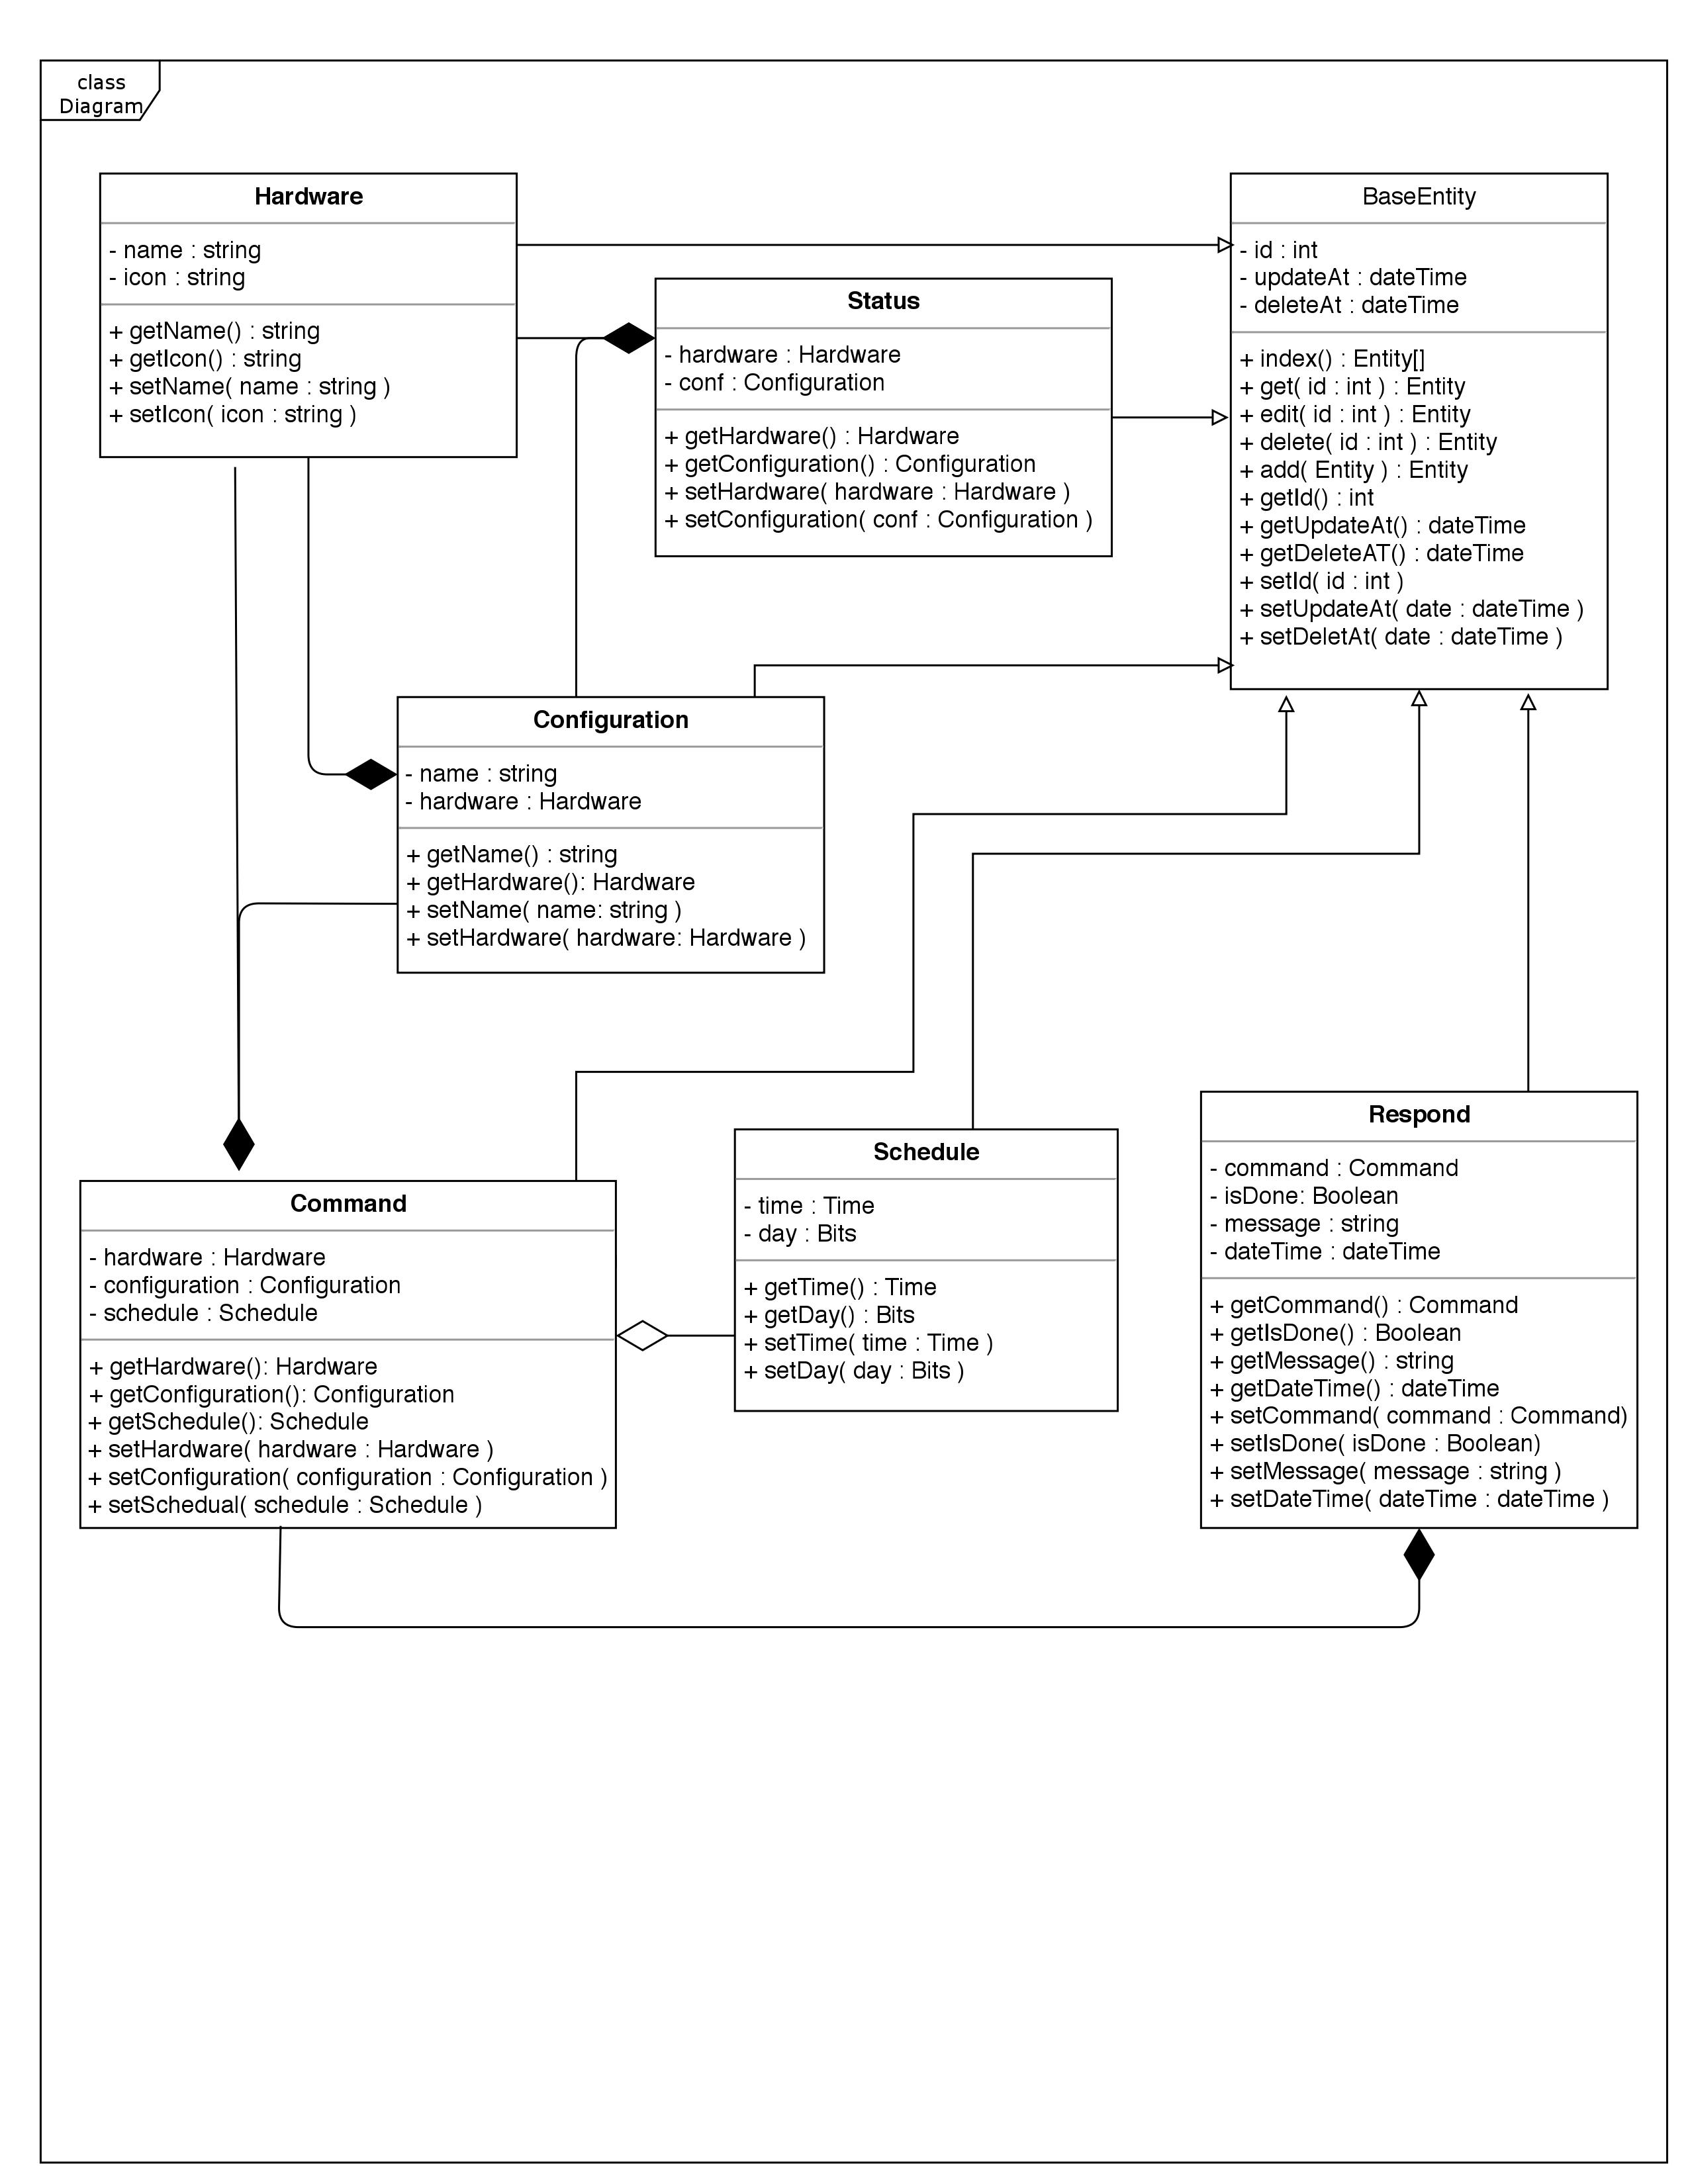
\includegraphics[width=\linewidth]{img/diagram_class.jpg}
					\end{figure}
				
		\newpage
	\begin{comment}
		usecase
		sequence
		desc
		
		ERD
			
	\chapter{System Design}
		\section{System Architecture}
		\section{User Interface Design}
		\newpage	
	\chapter{Implementation}
		\section{Implementation}
		\section{Implementation Requirements}
			\subsection{Software Requirements}
			\subsection{Hardware Requirements}
		\section{Implementation Detailed}
		\section{I/O Screens}
		\newpage	
	\chapter{Testing}
		\section{Testing}
		\section{Test Plan}
			\subsection{Unit Test}
			\subsection{Functional Test}
			\subsection{Acceptance Test}
		\section{Test Items}
			\subsection{Features to Be Tested}
			\subsection{Schedule of Test Actions}
			\subsection{Test Tasks}
		\section{Test Case}
		\section{Test Result}
		\newpage	
	\chapter{Conclusion}
		\section{Conclusion}
		\section{Evaluation}
		\section{Future Work}
	\newpage
	\end{comment}
	\bibliographystyle{ieeetr}


	\renewcommand{\bibname}{References}
	\addcontentsline{toc}{chapter}{References}
	\bibliography{References}


	\newpage
	\addcontentsline{toc}{chapter}{Appendices}
	\appendix
	

\end{document}
